\documentclass{standalone}
\usepackage{tikz}
\usetikzlibrary{patterns, positioning}


\begin{document}
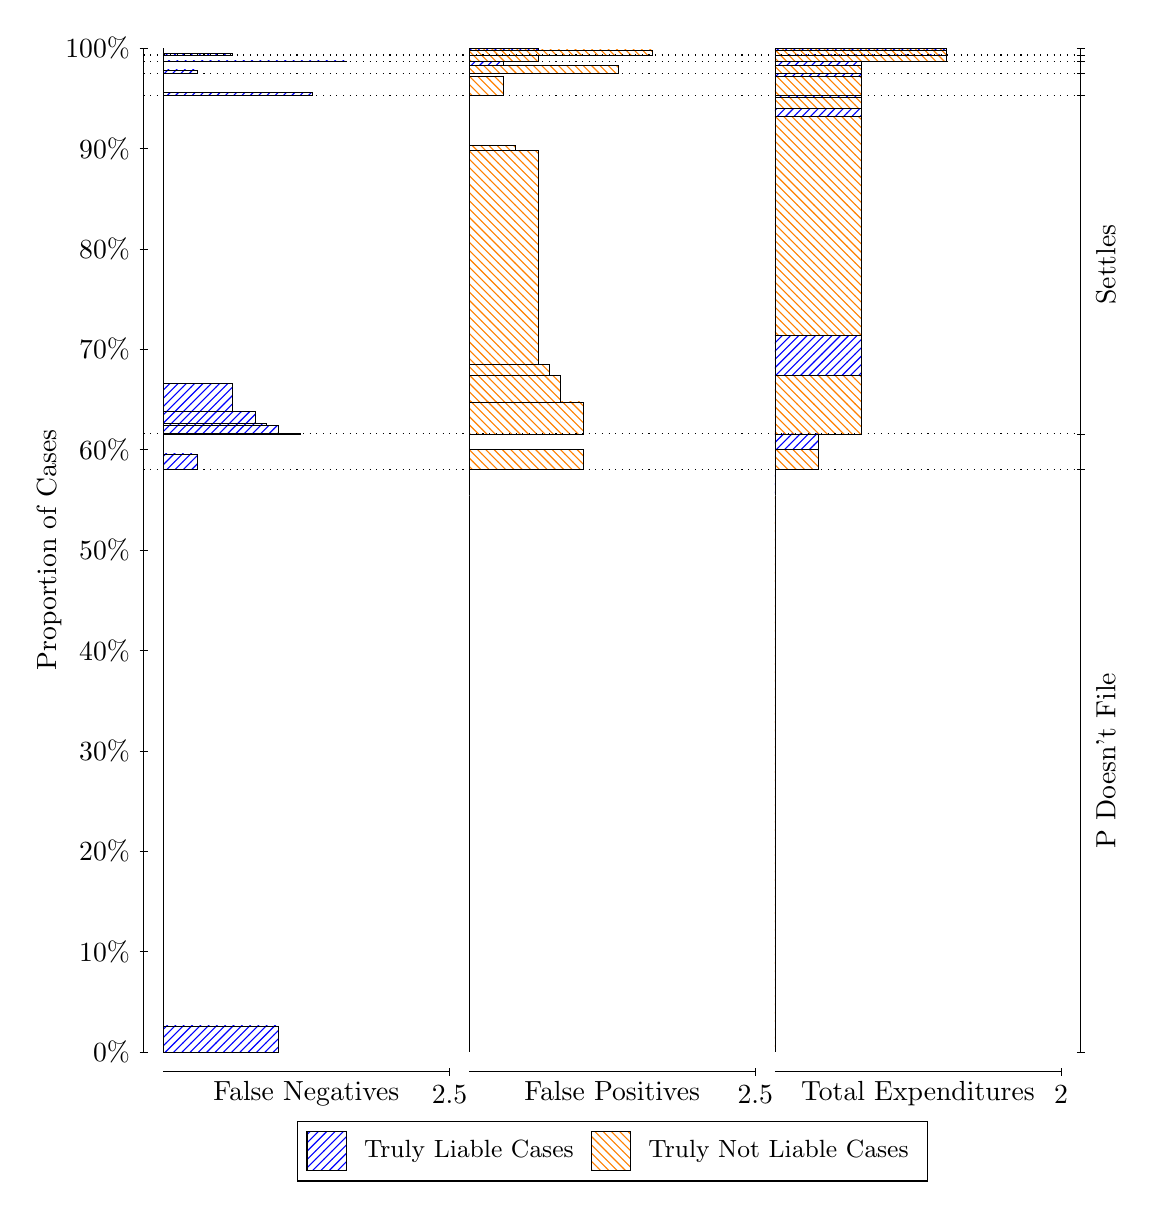
\begin{tikzpicture}
\draw[black, very thin] (1.5,1.75) -- (1.5,14.5);
\node[rotate=90, text=black, anchor=center] at (0.3, 8.125) {Proportion of Cases};
\draw[black, very thin] (1.45,1.75) -- (1.55,1.75);
\node[text=black, anchor=east] at (1.45, 1.75) {0\%};
\draw[black, very thin] (1.45,3.025) -- (1.55,3.025);
\node[text=black, anchor=east] at (1.45, 3.025) {10\%};
\draw[black, very thin] (1.45,4.3) -- (1.55,4.3);
\node[text=black, anchor=east] at (1.45, 4.3) {20\%};
\draw[black, very thin] (1.45,5.575) -- (1.55,5.575);
\node[text=black, anchor=east] at (1.45, 5.575) {30\%};
\draw[black, very thin] (1.45,6.85) -- (1.55,6.85);
\node[text=black, anchor=east] at (1.45, 6.85) {40\%};
\draw[black, very thin] (1.45,8.125) -- (1.55,8.125);
\node[text=black, anchor=east] at (1.45, 8.125) {50\%};
\draw[black, very thin] (1.45,9.4) -- (1.55,9.4);
\node[text=black, anchor=east] at (1.45, 9.4) {60\%};
\draw[black, very thin] (1.45,10.675) -- (1.55,10.675);
\node[text=black, anchor=east] at (1.45, 10.675) {70\%};
\draw[black, very thin] (1.45,11.95) -- (1.55,11.95);
\node[text=black, anchor=east] at (1.45, 11.95) {80\%};
\draw[black, very thin] (1.45,13.225) -- (1.55,13.225);
\node[text=black, anchor=east] at (1.45, 13.225) {90\%};
\draw[black, very thin] (1.45,14.5) -- (1.55,14.5);
\node[text=black, anchor=east] at (1.45, 14.5) {100\%};

\draw[black, very thin] (13.4,1.75) -- (13.4,14.5);
\draw[black, very thin] (13.35,1.75) -- (13.45,1.75);
\node[anchor=west] at (13.35, 1.75) {};
\draw[black, very thin] (13.35,9.1498) -- (13.45,9.1498);
\node[anchor=west] at (13.35, 9.1498) {};
\draw[black, very thin] (13.35,9.6009) -- (13.45,9.6009);
\node[anchor=west] at (13.35, 9.6009) {};
\draw[black, very thin] (13.35,13.9) -- (13.45,13.9);
\node[anchor=west] at (13.35, 13.9) {};
\draw[black, very thin] (13.35,14.174) -- (13.45,14.174);
\node[anchor=west] at (13.35, 14.174) {};
\draw[black, very thin] (13.35,14.33) -- (13.45,14.33);
\node[anchor=west] at (13.35, 14.33) {};
\draw[black, very thin] (13.35,14.412) -- (13.45,14.412);
\node[anchor=west] at (13.35, 14.412) {};
\draw[black, very thin] (13.35,14.5) -- (13.45,14.5);
\node[anchor=west] at (13.35, 14.5) {};

\draw[black, very thin, pattern color=blue, pattern=north east lines] (1.75,1.75) rectangle (3.2033,2.0808);
\draw[black, very thin, pattern color=orange, pattern=north west lines] (1.75,2.0808) rectangle (1.75,9.1498);
\draw[black, very thin, pattern color=blue, pattern=north east lines] (1.75,9.1498) rectangle (2.186,9.3455);
\draw[black, very thin, pattern color=orange, pattern=north west lines] (1.75,9.3455) rectangle (1.75,9.6009);
\draw[black, very thin, pattern color=blue, pattern=north east lines] (1.75,9.6009) rectangle (3.494,9.6083);
\draw[black, very thin, pattern color=blue, pattern=north east lines] (1.75,9.6083) rectangle (3.2033,9.7036);
\draw[black, very thin, pattern color=blue, pattern=north east lines] (1.75,9.7036) rectangle (3.058,9.7282);
\draw[black, very thin, pattern color=blue, pattern=north east lines] (1.75,9.7282) rectangle (2.9127,9.8878);
\draw[black, very thin, pattern color=blue, pattern=north east lines] (1.75,9.8878) rectangle (2.622,10.239);
\draw[black, very thin, pattern color=orange, pattern=north west lines] (1.75,10.239) rectangle (1.75,13.9);
\draw[black, very thin, pattern color=blue, pattern=north east lines] (1.75,13.9) rectangle (3.6393,13.932);
\draw[black, very thin, pattern color=orange, pattern=north west lines] (1.75,13.932) rectangle (1.75,14.174);
\draw[black, very thin, pattern color=blue, pattern=north east lines] (1.75,14.174) rectangle (2.186,14.221);
\draw[black, very thin, pattern color=orange, pattern=north west lines] (1.75,14.221) rectangle (1.75,14.33);
\draw[black, very thin, pattern color=blue, pattern=north east lines] (1.75,14.33) rectangle (4.0753,14.337);
\draw[black, very thin, pattern color=orange, pattern=north west lines] (1.75,14.337) rectangle (1.75,14.412);
\draw[black, very thin, pattern color=blue, pattern=north east lines] (1.75,14.412) rectangle (2.622,14.436);
\draw[black, very thin, pattern color=orange, pattern=north west lines] (1.75,14.436) rectangle (1.75,14.5);
\draw[black, very thin, pattern color=orange, pattern=north west lines] (5.6333,1.75) rectangle (5.6333,8.819);
\draw[black, very thin, pattern color=blue, pattern=north east lines] (5.6333,8.819) rectangle (5.6333,9.1498);
\draw[black, very thin, pattern color=orange, pattern=north west lines] (5.6333,9.1498) rectangle (7.0867,9.4053);
\draw[black, very thin, pattern color=blue, pattern=north east lines] (5.6333,9.4053) rectangle (5.6333,9.6009);
\draw[black, very thin, pattern color=orange, pattern=north west lines] (5.6333,9.6009) rectangle (7.0867,10.007);
\draw[black, very thin, pattern color=orange, pattern=north west lines] (5.6333,10.007) rectangle (6.796,10.341);
\draw[black, very thin, pattern color=orange, pattern=north west lines] (5.6333,10.341) rectangle (6.6507,10.479);
\draw[black, very thin, pattern color=orange, pattern=north west lines] (5.6333,10.479) rectangle (6.5053,13.198);
\draw[black, very thin, pattern color=orange, pattern=north west lines] (5.6333,13.198) rectangle (6.2147,13.262);
\draw[black, very thin, pattern color=blue, pattern=north east lines] (5.6333,13.262) rectangle (5.6333,13.9);
\draw[black, very thin, pattern color=orange, pattern=north west lines] (5.6333,13.9) rectangle (6.0693,14.142);
\draw[black, very thin, pattern color=blue, pattern=north east lines] (5.6333,14.142) rectangle (5.6333,14.174);
\draw[black, very thin, pattern color=orange, pattern=north west lines] (5.6333,14.174) rectangle (7.5227,14.283);
\draw[black, very thin, pattern color=blue, pattern=north east lines] (5.6333,14.283) rectangle (6.0693,14.33);
\draw[black, very thin, pattern color=orange, pattern=north west lines] (5.6333,14.33) rectangle (6.5053,14.405);
\draw[black, very thin, pattern color=blue, pattern=north east lines] (5.6333,14.405) rectangle (5.6333,14.412);
\draw[black, very thin, pattern color=orange, pattern=north west lines] (5.6333,14.412) rectangle (7.9587,14.476);
\draw[black, very thin, pattern color=blue, pattern=north east lines] (5.6333,14.476) rectangle (6.5053,14.5);
\draw[black, very thin, pattern color=orange, pattern=north west lines] (9.5167,1.75) rectangle (9.5167,8.819);
\draw[black, very thin, pattern color=blue, pattern=north east lines] (9.5167,8.819) rectangle (9.5167,9.1498);
\draw[black, very thin, pattern color=orange, pattern=north west lines] (9.5167,9.1498) rectangle (10.062,9.4053);
\draw[black, very thin, pattern color=blue, pattern=north east lines] (9.5167,9.4053) rectangle (10.062,9.6009);
\draw[black, very thin, pattern color=orange, pattern=north west lines] (9.5167,9.6009) rectangle (10.607,10.341);
\draw[black, very thin, pattern color=blue, pattern=north east lines] (9.5167,10.341) rectangle (10.607,10.851);
\draw[black, very thin, pattern color=orange, pattern=north west lines] (9.5167,10.851) rectangle (10.607,13.634);
\draw[black, very thin, pattern color=blue, pattern=north east lines] (9.5167,13.634) rectangle (10.607,13.737);
\draw[black, very thin, pattern color=orange, pattern=north west lines] (9.5167,13.737) rectangle (10.607,13.876);
\draw[black, very thin, pattern color=blue, pattern=north east lines] (9.5167,13.876) rectangle (10.607,13.9);
\draw[black, very thin, pattern color=orange, pattern=north west lines] (9.5167,13.9) rectangle (10.607,14.142);
\draw[black, very thin, pattern color=blue, pattern=north east lines] (9.5167,14.142) rectangle (10.607,14.174);
\draw[black, very thin, pattern color=orange, pattern=north west lines] (9.5167,14.174) rectangle (10.607,14.283);
\draw[black, very thin, pattern color=blue, pattern=north east lines] (9.5167,14.283) rectangle (10.607,14.33);
\draw[black, very thin, pattern color=orange, pattern=north west lines] (9.5167,14.33) rectangle (11.697,14.405);
\draw[black, very thin, pattern color=blue, pattern=north east lines] (9.5167,14.405) rectangle (11.697,14.412);
\draw[black, very thin, pattern color=orange, pattern=north west lines] (9.5167,14.412) rectangle (11.697,14.476);
\draw[black, very thin, pattern color=blue, pattern=north east lines] (9.5167,14.476) rectangle (11.697,14.5);
\draw[black, dotted] (1.5,9.1498) -- (13.4,9.1498);
\draw[black, dotted] (1.5,9.6009) -- (13.4,9.6009);
\draw[black, dotted] (1.5,13.9) -- (13.4,13.9);
\draw[black, dotted] (1.5,14.174) -- (13.4,14.174);
\draw[black, dotted] (1.5,14.33) -- (13.4,14.33);
\draw[black, dotted] (1.5,14.412) -- (13.4,14.412);
\draw[black, very thin] (1.75,1.5) -- (5.3833,1.5);
\node[text=black, anchor=north] at (3.5667, 1.5) {False Negatives};
\draw[black, very thin] (5.3833,1.45) -- (5.3833,1.55);
\node[text=black, anchor=north] at (5.3833, 1.45) {2.5};

\draw[black, very thin] (5.6333,1.5) -- (9.2667,1.5);
\node[text=black, anchor=north] at (7.45, 1.5) {False Positives};
\draw[black, very thin] (9.2667,1.45) -- (9.2667,1.55);
\node[text=black, anchor=north] at (9.2667, 1.45) {2.5};

\draw[black, very thin] (9.5167,1.5) -- (13.15,1.5);
\node[text=black, anchor=north] at (11.333, 1.5) {Total Expenditures};
\draw[black, very thin] (13.15,1.45) -- (13.15,1.55);
\node[text=black, anchor=north] at (13.15, 1.45) {2};

\node[text=black, centered, rotate=90] at (13.72, 5.4499) {P Doesn't File};

\node[text=black, centered, rotate=90] at (13.72, 11.751) {Settles};





\draw (7.449999999999999,1.5) node[draw=none] (baseCoordinate) {};
\begin{scope}[align=center]
        \matrix[scale=0.5, draw=black, below=0.5cm of baseCoordinate, nodes={draw}, column sep=0.1cm]{
            \node[rectangle, draw, minimum width=0.5cm, minimum height=0.5cm, pattern color=blue, pattern=north east lines] {}; &
            \node[draw=none, font=\small, text=black] (B) {Truly Liable Cases}; &
            \node[rectangle, draw, minimum width=0.5cm, minimum height=0.5cm, pattern color=orange, pattern=north west lines] {}; &
            \node[draw=none, font=\small, text=black] (B) {Truly Not Liable Cases}; \\
            };
\end{scope}

\end{tikzpicture}
\end{document}